\documentclass[]{ctexbook}

\usepackage[a4paper,left=2cm,right=2cm,top=2cm,bottom=2cm]{geometry}
\usepackage[dvipsnames]{xcolor}
\usepackage[most]{tcolorbox}
\usepackage{amsmath}
\usepackage{listings}
\usepackage{pdfpages}
\usepackage{hyperref} 

\definecolor{codegreen}{rgb}{0,0.6,0}
\definecolor{codegray}{rgb}{0.5,0.5,0.5}
\definecolor{codepurple}{rgb}{0.58,0,0.82}
\definecolor{backcolour}{rgb}{0.95,0.95,0.92}

\lstset{
    backgroundcolor=\color{backcolour},
    commentstyle=\color{codegreen},
    keywordstyle=\color{magenta},
    numberstyle=\tiny\color{codegray},
    stringstyle=\color{codepurple},
    basicstyle=\ttfamily\fontsize{9}{11}\selectfont,  % 调整这里的字体大小和行高
    numbers=left,
    stepnumber=1,
    numbersep=5pt,
    abovecaptionskip=1em,
    breaklines=true,  
    breakatwhitespace=true,  
    captionpos=b,  
    keepspaces=true,  
    showspaces=false,  
    showstringspaces=false,
    showtabs=false,
    tabsize=2,
}

\newcommand{\citebox}[1]{
    \begin{center}
    \begin{tcolorbox}[colback=gray!10,%gray background
                      colframe=black,% black frame colour
                      width=15cm,% Use 8cm total width,
                      arc=1mm, auto outer arc,
                      boxrule=0.5pt,
                     ]
    #1
    \end{tcolorbox}
    \end{center}
}


\title{COMPSCI 742 押题}
\author{Bo Pang/庞礴}
\date{Last Update: \today}

\ctexset{
	part = {
		format+=\heiti
	},
    part/name = {第, 编},
    part/number = {\Chinese{part}},
    chapter/name = {第, 章},
    chapter/number = { \arabic{chapter}},
    chapter = {
		format+=\heiti
	},
    section = {
		format+=\heiti
	},
	subsection = {
		format+=\heiti
	},
	subsubsection = {
		format+=\heiti
	},
    paragraph = {
		format+=\heiti
	}
}


\begin{document}
\maketitle
\tableofcontents

\part{网络测量}

\chapter*{必读书目}

\section{Web workload characterization}
\section{Pinging in the rain}
\section{Modern website complexity}
\section{Comparative analysis of Web and P2P traffic}
\section{Interference effects in Wi-Fi networks}


\chapter{网络测量}

\section{网络测量中的概念}

互联网测量可根据网络监控器的位置(边缘网络与核心网络)、使用的测量/分析工具(基于硬件与基于软件)、探测机制(被动与主动)以及视点数量(单视点与多视点)进行分类。

\subsection{了解主动与被动等测量方法,以及边缘与核心等有利位置}

被动网络测量是通过监听通过路由器或主机的所有流量来进行的。主动测量包括生成从一台主机到另一台主机的特殊探测流量。探测流量可能包含几乎没有有效载荷的小型 UDP 数据包。

注意,Google Analytics被视为主动测量。

\subsection{给定一个场景,确定测量方法和有利位置}
在对WWW2007网站进行测量时,采用了被动测量和主动测量两种方法。

因为本研究收集并分析了服务器端数据和客户端数据。在服务器端,数据是从服务器日志中收集的,而客户端数据则是从 Google Analytics 服务中收集的。收集和分析服务器日志是观察服务器的一种方式,因此是被动的。

使用 Google Analytics 服务会在网页中注入 JS 部分,从客户端收集数据。它不需要用户额外参与或干预,但会主动向 Google Analytics 服务发送数据。因此,这是一种主动测量。

视点包括服务器端和客户端,它们都是边缘视点。因为服务器端和客户端都处于互联网网络的边缘。

这项工作考虑了多种观点。研究采用了服务器端和客户端测量技术来描述网站访问者的使用行为。在服务器端,研究分析了服务器的使用情况和流量。在客户端,还研究了多种用户行为,如提示、浏览网站的偏好和页面深度等。

本次测量研究进行了离线分析。研究分析了网络服务器上的文件,以研究服务器的性能,而 Google Analytics 则报告了客户端的行为。所有分析都是离线完成的。

测量中使用到的软件工具主要有:访问日志、文件列表、谷歌分析服务、Cookie强化日志、服务器插件。
\section{网站的复杂性}

\subsection{研究的意义}
这项研究的意义在于揭示了网站复杂性对用户体验的影响,尤其是页面加载时间对用户满意度的直接影响。

\subsection{影响网站性能的因素及其原因}

\subsubsection{内容层面}

\begin{itemize}
	\item \textbf{对象数量和大小:}研究发现,网站加载的对象数量是影响页面渲染和加载时间的最重要因素。在所有等级范围内,网页请求的对象数量中位数超过40个,20\% 的网页请求的对象数量超过100个。新闻网站加载的对象数量明显多于其他网站。对象的大小也是一个重要的考量,但其影响相对较小(页面8)。每个对象都需要单独的HTTP请求,因此对象数量的增加会导致更多的网络延迟和服务器处理时间,从而增加页面加载时间;而大对象(如高分辨率图片或大型JavaScript文件)会占用更多的带宽,导致加载时间增加。
	\item \textbf{内容类型:}网站加载的内容类型也影响性能。各种内容类型在不同等级范围内的贡献相似。图片在对象比例中占主导地位,但在字节比例中占较小比例。儿童和青少年网站的 Flash 内容比例明显高于其他网站。不同类型的内容(如Flash或JavaScript)可能需要额外的客户端处理时间,这会影响页面的可用性和响应速度。
\end{itemize}

\subsubsection{服务层面}
\begin{itemize}
	\item \textbf{服务器数量:}25-55\%的网站从至少10个服务器加载内容。新闻网站从明显多于其他网站的服务器获取内容。服务器数量增加可能会导致更多的网络延迟和更复杂的服务器处理,这可能会导致加载时间的不确定性和波动。此外,客户端可能需要开启多个HTTP/TCP连接到许多不同的服务器,这也会增加页面的加载时间。
	\item \textbf{非源内容(服务器、对象、时间):}超过60\%的网站从至少5个非源源加载内容。非源内容贡献了超过35\%的下载字节。然而,非源内容对下载时间的影响相对较低,因为浏览器的优化减少了它们的影响(页面1、2)。图片是由源码提供的主要对象类型,但 Javascript 占非源码对象的很大一部分。广告和分析服务是最常见的非源对象,而内容分发网络(CDNs)则贡献了大部分字节。这些第三方服务的集成对网站性能有显著影响(页面4)。由于浏览器需要解析和执行来自不同源的内容,这可能会引入额外的延迟。尽管浏览器优化可以减少这种影响,但过多的非起源内容仍然可能导致性能问题。
\end{itemize}




\chapter{齐普夫定律}
在论文《1.3 Characterization of Content Delivery Applications》、《3.1* Workload Characterization of a Large Systems Conference Web Server》中,作者都提到了齐普夫分布。

论文《7.4 A Tale of the Tails: Power-laws in Internet Measurements》中,详细介绍了齐普夫定律。论文揭示了互联网测量中的幂律。幂律分布中的“重尾”和“长尾”现象称作“尾巴的故事”。在互联网测量中,这些分布常常表现出尾部的数据值比正态分布或指数分布中的要多,这意味着在分布的尾部有一些非常大的值出现的概率非常高。

\begin{itemize}
	\item \textbf{重尾(Heavy Tails):}如果一个概率分布的尾部不是指数级地减少,那么这个分布就被称为重尾。重尾分布强调了大值的存在,这些较少出现的大值的变化对分布的影响比频繁出现的小值的变化更大。

	\item \textbf{长尾(Long Tails):}长尾现象是幂律关系的一个表现,它体现了低频事件在统计上比高斯分布要多得多。例如,搜索引擎中使用的关键词就表现出长尾特性,即存在一长串不常用的关键词,尽管每个关键词的使用频率不高,但它们加起来可能占搜索引擎看到的关键词搜索的很大一部分。
\end{itemize}

\section*{幂律分布}

幂律特性通常出现在高方差分布中,在这种分布中,观测值的数量级跨度很大,尤其是在分布有明显偏斜的情况下。与广泛用于电信系统数学建模的指数分布相比,幂律分布的衰减速度更慢。幂律的存在表明,任意大数值可能以不可忽略的概率出现,因此,如果大型数据集中存在足够多的此类样本,与其将这些极端值视为 "异常值 "而忽略不计,不如研究其统计普遍性。

幂函数以$f(x)=\alpha \times x^{-\eta}$的形式出现。其中,$\alpha$和$\eta$是正数常量,$\eta$称为标度指数(scaling exponent)。对幂函数两边取对数得出 $\log (f(x)) = -\eta \log (x) + \log (\alpha)$。这个表达式呈现线性关系,斜率为$-\eta$,y轴截距为$\log (\alpha)$。在对数-对数标尺上绘制时,该函数显示为一条直线。这种现象通常被认为是幂律关系的显著特征。

幂律分布是在计算机科学文献中常用来描述某些数据集特性的一种分布。幂律分布的特点是,当你观察数据集中的大数值时,数据的分布遵循一个幂函数的形式。这里的幂函数表示为 $f(x)\sim  x^{−\eta}$,其中 $\sim$ 符号表示随着 $x$增加到很大的值时(趋向于无穷大),$f(x)$ 与 $x^{−\eta}$ 的比值趋近于某个正常数$c$。

当$ x $趋于无穷大时(即在数据集的``尾部''),比例 $f(x)/x^{−\eta}$ 趋向于一个正常数$c$。在实际应用中,这意味着数据的大值不会像正态分布那样迅速减少,而是以一种可预测的方式缓慢地减少。这是幂律分布的一个关键特征,通常用来描述社会、科技和自然现象中的许多类型的数据。在数据的尾部,即我们关注较大数值时,这个性质特别显著,因此这部分被称为“分布的尾部”。

幂律在许多自然发生的现象中被观察到(例如,地震、降水、地形),以及在许多人类行为中(例如,引文、城市人口、财富)。在信息系统的许多方面也观察到幂律,包括软件系统和计算机网络。早期例子包括虚拟内存系统中的内存引用行为、数据库查询以及文件系统中的文件使用模式。互联网和网络的几个特性也被声称表现出幂律特性,例如网站的访问者数量、网页的超链接数量、网页对象的大小、互联网上路由器的链接数量、在线社交网络上用户的朋友数量。

\subsubsection{帕累托分布}

帕累托分布(Pareto Distribution),这是一种在互联网流量测量中常见的幂律分布(power-law distribution)。帕累托分布可以用来描述那些大事件发生概率低但影响巨大的现象,常见于经济、社会科学和许多自然现象中。

在描述帕累托分布时,通常会用到互补累积分布函数(CCDF),它用来表示一个事件发生的概率大于某个值$x$。数学上,CCDF用$P[X>x]$ 表示,并且满足与$−\kappa$成反比,这里的$\kappa$是形状参数(shape parameter)。这个性质表明,随着$x$的增加,发生大于$x$的事件的概率以 x 的$−\kappa$次幂衰减。

在双对数坐标轴(doubly logarithmic scales)上绘制 CCDF 时,如果数据遵循幂律分布,那么会在图上显示为一条直线。确定一个数据集是否遵循对数正态、幂律或其他相关分布并不容易,识别的金标准是在双对数坐标上看到一条直线。

此外,幂函数的积分本身也是一个幂函数,这意味着如果你对帕累托分布的密度函数进行积分,你得到的累积分布函数(CDF)仍然是幂律形式的。因此,可以很容易地展示帕累托分布和幂律分布之间的关系,通过$\kappa = \eta −1$这一关系式,其中$\eta$是之前讨论的幂律分布的指数。

指数分布(exponential distribution)和对数正态分布(lognormal distribution)的尾部行为(即大值事件的概率衰减)和帕累托分布是不同的。帕累托分布的尾部比指数分布更厚,也就是说,在大事件发生的概率方面下降得更慢。
\section{什么是齐普夫定律}

\subsubsection{GPT的解释}

齐普夫定律(Zipf's Law)是由美国语言学家乔治·金斯利·齐普夫(George Kingsley Zipf)提出的一种经验法则。它描述了一种在自然语言文本中出现的词频分布现象,即在给定的语料库中,任何词的频率与它在频率表中的排名成反比。

具体来说,齐普夫定律指出,语料库中最常见的词出现的次数大约是第二常见的词的两倍,是第三常见的词的三倍,以此类推。换句话说,第n个最常见的词在语料库中出现的频率大致成1/n的规模。这个定律在自然语言的各种现象中都有体现,如单词的使用频率、城市人口排名、网站访问量等。

数学上,齐普夫定律可以用以下的公式表示:
\[f(n) = \frac{C}{n^a}\]
这里的$f(n)$表示排名为n的项的频率,$C$是一个常数,$a$通常接近于1。

齐普夫定律不仅仅适用于语言学,它在许多自然和社会科学领域都有广泛的应用,显示出一种普遍的幂律分布特征。例如,它也被用来描述城市规模、公司规模、收入分布等的统计特性。这个定律的一个有趣的特点是,尽管它非常简单,但它却能非常准确地描述现实世界中的各种现象。

\subsubsection{论文7.4的解释}

幂律的另一个经典例子是齐普夫分布,它最早用于模拟书面文本中的词频,后来又被用于模拟图书馆图书、电影租赁和网络对象的偏斜流行度。齐普夫分布是一种离散分布,在等级-频率域中由齐普夫定律定义,该定律指出,当项目按受欢迎程度降序排列(R)时,项目的频率(F)与项目的等级成反比。


\section{齐普夫定律的数学表示}

齐普夫分布是一种离散分布,在等级-频率域中由齐普夫定律定义:如果我们将一些项目按照它们的流行度排名,排在第$R$位的项目的频率$F$和它的排名$R$的关系可以用下面的公式表示:

\[F \propto R^{-\theta}\]

\section{齐普夫定律的参数}

在一个对数-对数排名-频率图上,齐普夫分布呈现为一条直线,这条直线的斜率是$-\theta$。在这种图上,两个坐标轴(排名和频率)都是对数刻度,因此原本呈幂律分布的关系在这样的图上显示为直线关系。$\theta$通常接近$1$,但也可以有不同的值。意味着排名每增加10倍(一个对数单位),频率会减少到原来的大约$1/10$。当$\theta=1$时,我们得到一个纯粹的齐普夫分布。

在实际的互联网度量中,可能会观察到齐普夫分布的“退化形式(Degenerate forms)”,这种情况下分布的行为是分段线性的,或者说只有图中的一部分是线性的。这意味着实际观察到的数据可能在某些排名区间内遵循齐普夫分布,在其他区间则不遵循。

例如,人们发现在点对点文件分享系统中,文件的流行度呈现出齐普夫分布的特征,但最受欢迎的文件与预期的直线有所偏离。这种偏离可能是因为用户通常按照“最多获取一次”的方式分享文件,也就是说,用户一旦下载了某个文件,就不太可能再去下载同一个文件,这导致了最流行的文件的实际频率低于齐普夫分布所预期的频率。

\subsubsection{齐普夫分布与帕累托分布的关系}

齐普夫分布可视为帕累托分布的离散解释。它可以通过变换帕累托分布的坐标轴来表示。因此,齐普夫分布可以写成:$R \propto F^{\frac{-1}{\theta}}$。也就是说,齐普夫分布中的$\theta$、帕累托分布中的$\kappa$、幂律分布中的$\eta$的关系为:
\[\kappa = \eta - 1 = \frac{1}{\theta}\]

这个关系表明,这些不同的分布实际上是通过参数相互转换的不同表达方式。

这表明在齐普夫分布中,少数非常流行的项目会得到大量的引用,体现了一个强烈的倾斜或偏态分布。在许多现实世界的数据集中,通常是小部分的元素占据了大部分的活动或资源。这是齐普夫分布的一个典型特征,也是帕累托法则的表现。

形状参数$\theta$决定了分布的倾斜程度。不同的$\theta$值将导致不同程度的倾斜。在许多实证研究中观察到了类似的倾斜现象,例如文中未给出的图2,可能展示了某些主机对Web服务器的请求情况,其中少数主机发起了大多数请求。这种现象在文献中通常被称为帕累托法则、帕累托原理或者80/20规则,即20\%的原因往往会产生80\%的结果。

\begin{figure}[h]
    \centering
    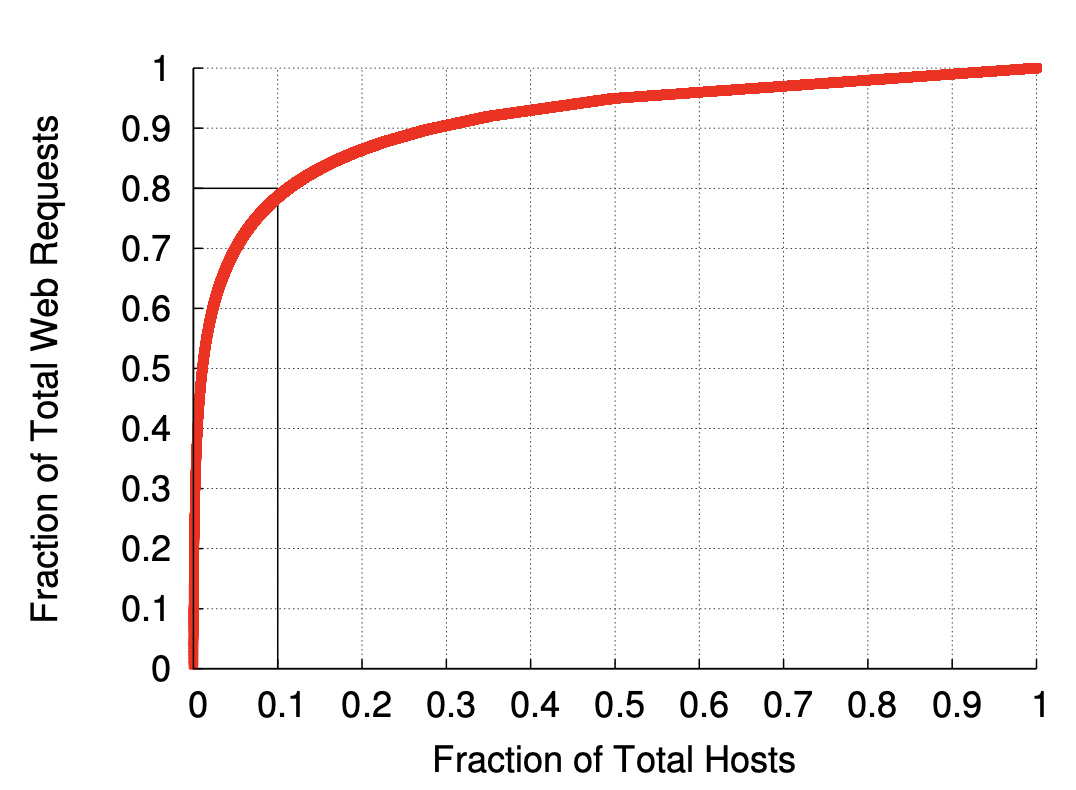
\includegraphics[width=5cm]{res/zipfex.png}
    \caption{Fig. 2. 帕累托原则:图中显示的是 WWW 2007 会议网络服务器在一年时间内的请求分布情况。我们观察到,排名前10\%的主机占了网络请求总量的80\%。这体现了帕累托原则,即大部分网络请求是由少数主机发出的。}
\end{figure}

\section{从图表中识别齐普夫定律并计算其参数}
\begin{figure}[h]
    \centering
    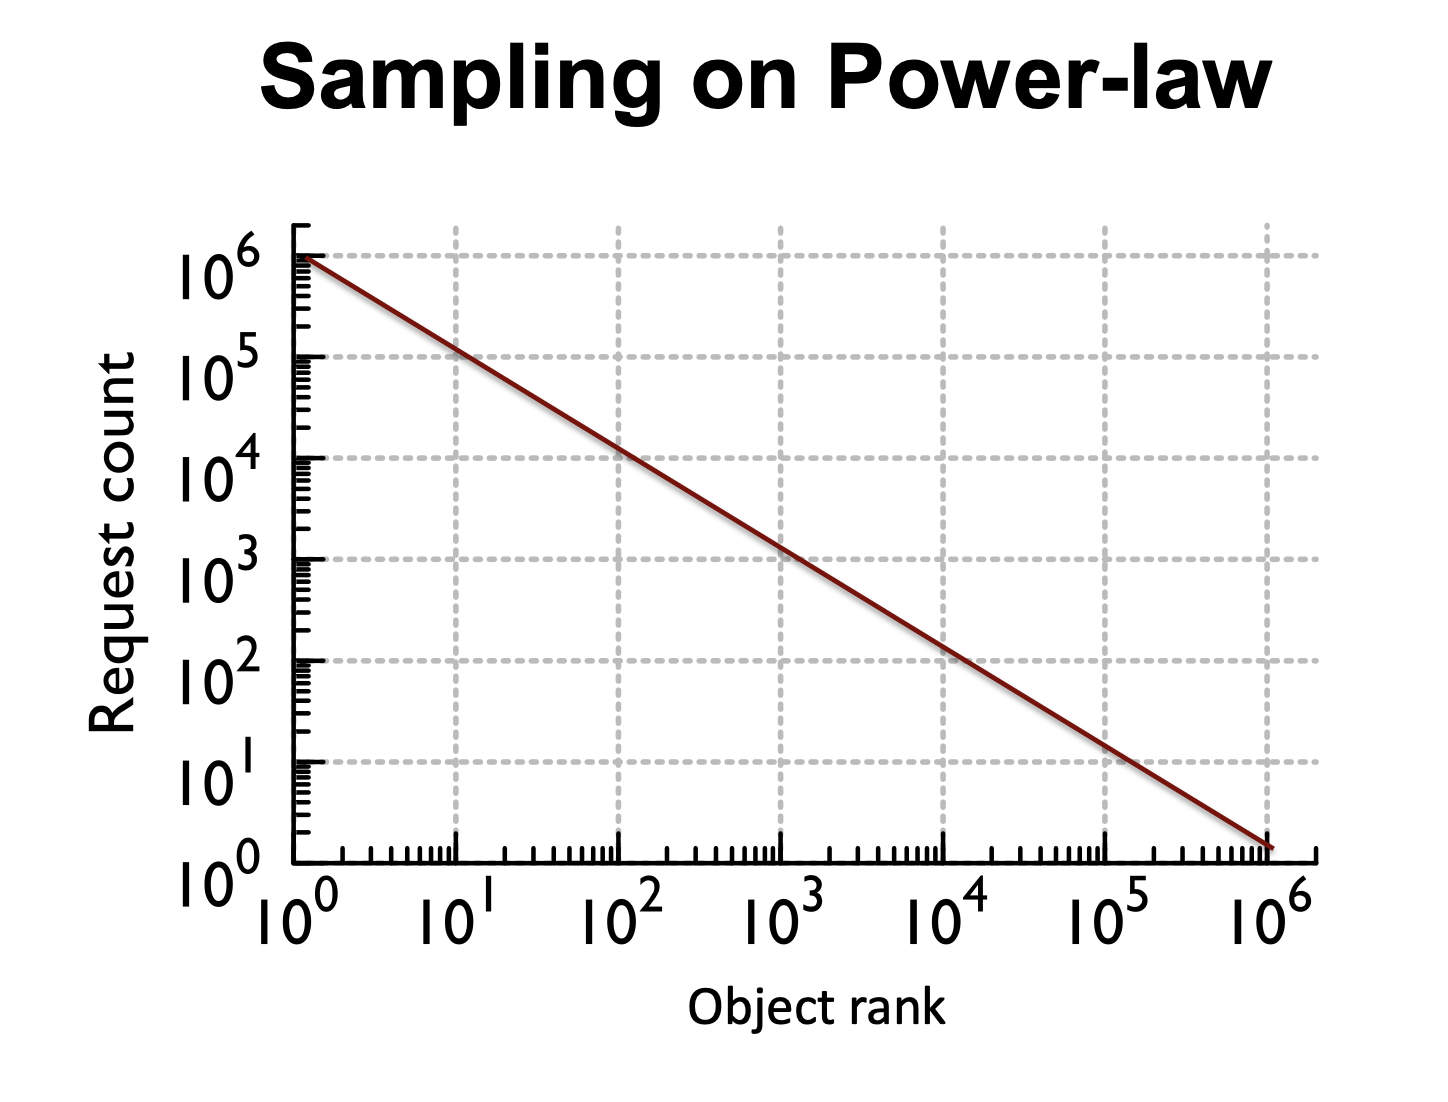
\includegraphics[width=5cm]{res/facebookpowerlaw.png}
    \caption{从图表中识别齐普夫定律并计算参数}
\end{figure}

在双对数坐标纸上绘制数据,即对数-对数图表。横轴为元素的排名($R$),纵轴为相应的频率($F$)。对数变换是为了线性化幂律关系,齐普夫定律预测这样的图应该呈现出一条直线。

对数据点进行线性拟合,以获得最佳拟合直线。这条线的斜率(在对数-对数图上)将与齐普夫分布的参数$\theta$相关。

斜率$m$通常会是负数,因为随着排名的增加,频率通常会下降。在齐普夫定律中,这个斜率$m$与$\theta$相关,通常有$m=−\theta$。因此,通过测量这个斜率,你可以计算出$\theta=−m$。
\section{齐普夫定律的含义}

在互联网测量中,齐普夫定律的应用包括但不限于Web缓存的有效性,它依赖于Web对象及其大小的非均匀流行度分布。Web访问已被证明遵循齐普夫定律,这在Web缓存架构的设计中非常重要,因为它允许设计者计算出近似的缓存大小以实现期望的命中率。适当的缓存大小和适当的替换策略可以实现高缓存命中率。齐普夫定律对于预测对象被访问的概率也很有用。

\subsection{Facebook Haystack 系统的分布式缓存案例研究}

Facebook将些照片存储在专门用于存储照片的Haystack机器上。但同时,还有一个深层次且分布式的照片服务堆栈,具备多层缓存,以便向人们传递照片,让他们能够查看这些照片。

照片服务堆栈有四个层次:浏览器缓存、边缘缓存、源缓存和Haystack后端。堆栈的第一层是人们机器上的浏览器缓存。如果有人最近查看或下载了一张照片,那么这张照片很可能在他们的浏览器缓存中,他们可以从本地检索到它。否则,他们的浏览器将向互联网发送一个HTTPS请求。该请求将被路由到我们的CDN合作伙伴之一,或者到Facebook的许多边缘缓存之一,这些缓存位于互联网的出口点(PoPs)。 (在论文和这篇博文中,我们关注的是在Facebook控制的堆栈中发生的情况。)请求被路由到的特定边缘缓存被编码在请求的URL中。如果请求的照片在边缘缓存中存在,则将照片返回给用户的浏览器,并将其存储在本地缓存中。如果照片在边缘缓存中不存在,则从源缓存中请求照片。源缓存是一个分布在多个数据中心(如Prineville、Forest City和Lulea)的单个缓存。来自边缘缓存的请求会根据所请求照片的ID路由到源缓存中的主机。这意味着对于单个图片,来自所有边缘缓存的源缓存请求都将被引导到同一个服务器。如果所请求的照片在源缓存中存在,它将通过边缘缓存返回给用户,而边缘缓存现在将存储该照片。如果所请求的照片不存在,则会从Haystack后端获取。Haystack后端存储所有照片,因此可以在这一层满足所有请求。来自源缓存的请求通常由同一数据中心的Haystack机器处理。如果由于某种原因本地的Haystack机器不可用,源缓存将从另一个数据中心的Haystack机器请求照片。无论哪种情况,照片都会沿着缓存层逐层存储并返回:源缓存,边缘缓存,然后是浏览器缓存。

在这项研究中,我们收集了一个月的请求跟踪数据,来自非移动用户,这些请求是用由Facebook控制的堆栈完全提供的确定性照片的子集。该跟踪数据捕获了堆栈的所有层次,包括客户端浏览器缓存中的命中和未命中。所有的分析和模拟都是基于这一跟踪数据进行的。根据我们的追踪,我们确定了每个层的命中率以及通过每个层传输的总请求比例。每个层都显著减少了流量量,使得Haystack后端只需要提供所请求照片的9.9\%。

\subsubsection{流行度分布的变化}

众所周知,网络上对象的受欢迎程度往往遵循幂律分布。我们的研究证实了这一点,同时展示了随着我们在系统层级中下降,这种分布如何发生变化。我们统计了每个层级中每张照片的请求数量,按照受欢迎程度进行排序,并在对数-对数尺度上绘制了图表。这种幂律关系在这个尺度上呈现为线性关系,\textbf{也就是齐普夫分布。}

\begin{figure}[h]
    \centering
    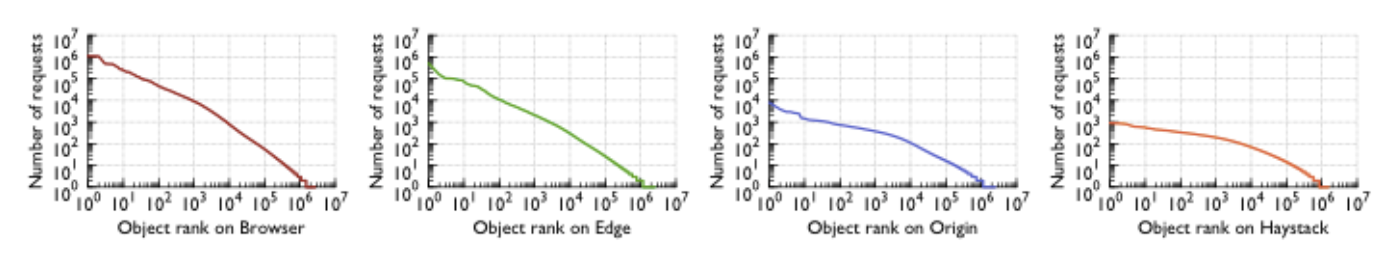
\includegraphics[width=16cm]{res/fb1.png}
    \caption{齐普夫分布随系统层级的下降的变化}
\end{figure}

随着我们向下移动堆栈,齐普夫分布的$\theta$参数逐渐减小并趋于平缓。

\subsection{不同缓存级别的内容受欢迎程度如何变化?}

\begin{figure}[h]
    \centering
    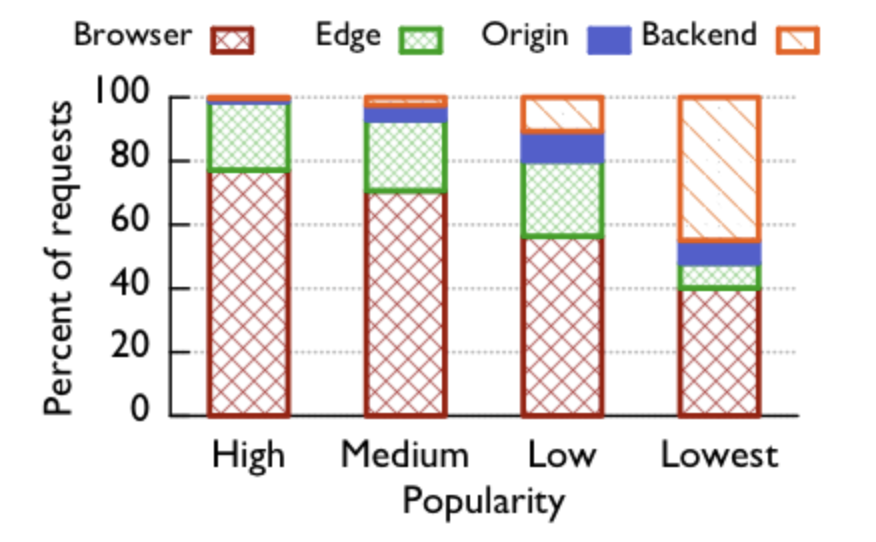
\includegraphics[width=9cm]{res/fb2.png}
    \caption{不同缓存级别的内容受欢迎程度 }
\end{figure}
缓存的主要作用是多次提供最受欢迎的内容。为了量化这一点在Facebook的堆栈中的真实程度,我们将照片分成了不同的受欢迎程度组。组“高”包含了最受欢迎的1,000张照片,组“中”包含接下来的9,000张最受欢迎的照片,组“低”包含接下来的90,000张最受欢迎的照片,而组“最低”则包含了在我们追踪的照片子集中最不受欢迎的2.5百万张照片。每个组大约占用户请求的25\%。这张图显示了这四个组中每个层级所提供的请求的百分比。

正如预期的那样,浏览器和边缘缓存对于我们的跟踪中最受欢迎的照片非常有效,但对于不太受欢迎的群体逐渐减少效果。源缓存的最大效果主要体现在受欢迎度较低的群体上,这也符合我们的直觉。更受欢迎的照片将更早地在浏览器和边缘层中有效地缓存。不太受欢迎的照片请求太少,无法有效地缓存。


\chapter{Wi-Fi环境干扰效应}
Wi-Fi 网络采用 IEEE 802.11 协议。由于使用的2.4GHz频段是未授权的,因此可供多种设备(Wi-Fi 和非 Wi-Fi 设备)使用,必然会造成相互干扰。802.11协议被认为是一种有礼貌的协议,因为 802.11 设备只有在感觉到射频信道空闲时才会进行传输。可微波炉等非 Wi-Fi 设备对该协议视而不见。无论信道是否空闲,这些设备都会进行传输。

我们使用现成的无线频谱分析仪来了解非 Wi-Fi 设备如何影响 Wi-Fi 网络的运行。通过受控实验,我们分析了六种非 802.11 设备的干扰特性。其中五个是无意干扰设备:一个微波炉、两个无绳电话(一个模拟和一个数字)、一个模拟无线摄像头和一个蓝牙耳机。我们还评估了一个有意干扰器,即无线干扰器,以进行比较。除了捕捉这些设备的基本特性外,我们还测量、量化和讨论了它们对数据、视频和语音流量的干扰影响。最后,我们通过对一个运行中的校园网络进行被动测量,试图了解干扰对网络的影响。

结果表明,在无意干扰中,微波炉、模拟无绳电话和无线摄像头对 Wi-Fi 网络的影响最大。
由于微波信号具有宽带干扰特性,因此在近距离内会影响多个 Wi-Fi 信道,但在较远距离内仍会产生影响。模拟无绳电话和无线摄像头是持续的窄带干扰源,它们使用的任何信道都会完全屏蔽 Wi-Fi 服务。数字无绳电话和蓝牙耳机由于其跳频特性,对 Wi-Fi 的影响微乎其微。通过对生产网络的测量,我们发现校园网络中存在大量非 Wi-Fi 设备,这些设备会对网络中的干扰水平产生重大影响。例如,在一天中的某些时段,几乎 80\% 的信道都可能被干扰器占用,而且经常可以看到一些干扰设备几乎一直处于活动状态(在后台)。

\section{物理层干扰特征}

我们使用频谱图和占空比来描述物理层干扰的特征。

\subsection{Spectrogram}

频谱图是\textbf{射频功率水平}在频谱中随时间变化的表示。
频谱图中的每条垂直线都表示射频功率与频率的函数关系,测量时间间隔为1秒。频谱图提供了频域射频功率的时间视角。

\subsubsection{Wi-Fi信道的结构}

Wi-Fi 信道分为 14 个重叠信道,每个信道的频谱带宽为 22 兆赫。图 2 展示了 2.4 千兆赫频段的 Wi-Fi 信道。图中显示了每个 Wi-Fi 信道的中心频率。相邻信道之间相隔 5 兆赫,但信道 14 除外,其中心频率与信道 13 相隔 12 兆赫。单个信道可同时处理 50 个或更多用户。Wi-Fi 信道的使用由各国的国家监管机构管理。在北美,只有前 11 个信道可供使用。在世界其他地区,前 13 个信道可供使用。

\begin{figure}[h]
    \centering
    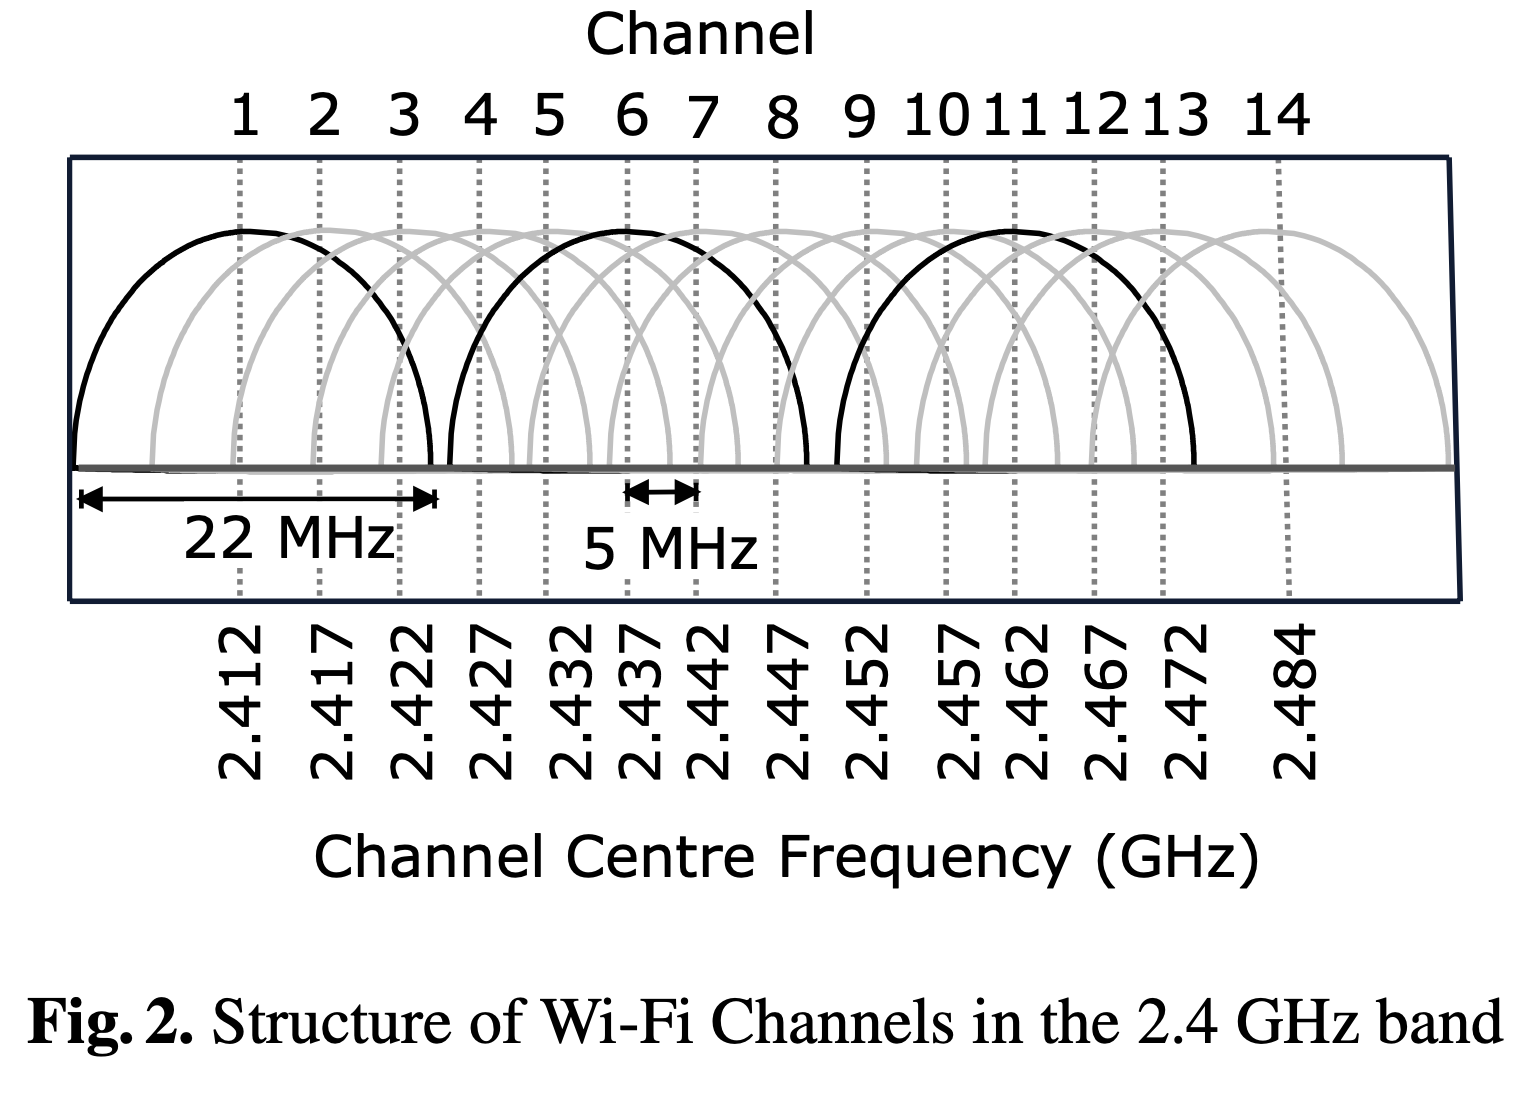
\includegraphics[width=9cm]{res/wifi3.png}
    \caption{Wi-Fi信道的结构}
\end{figure}

为避免干扰,无线无线电设备应在非重叠信道上运行,即信道之间至少相隔 22 兆赫。例如,如果两个无线接入点在一个无线小区的同一信道上运行,那么它们的信号就会相互干扰。这同样适用于任何其他辐射设备,如微波炉或无绳电话。从图 2 中我们可以看到,下列信道组合不会相互重叠: {1, 6, 11}、{2, 7}、{3, 8}、{4, 9}和{5, 10}。信道 1、6 和 11 是 Wi-Fi 部署中最常用的非重叠信道。

\subsection{Dutycycle}
占空比测量\textbf{频谱中的射频功率}。
在这项工作中,占空比是通过测量射频信号高于本底噪声 20 dBm 的时间百分比来计算的。占空比是射频功率对网络性能影响的指标。
\section{使用频谱图和占空比衡量Wi-Fi流量干扰}

\subsection{频谱图}

\begin{figure}[h]
    \centering
    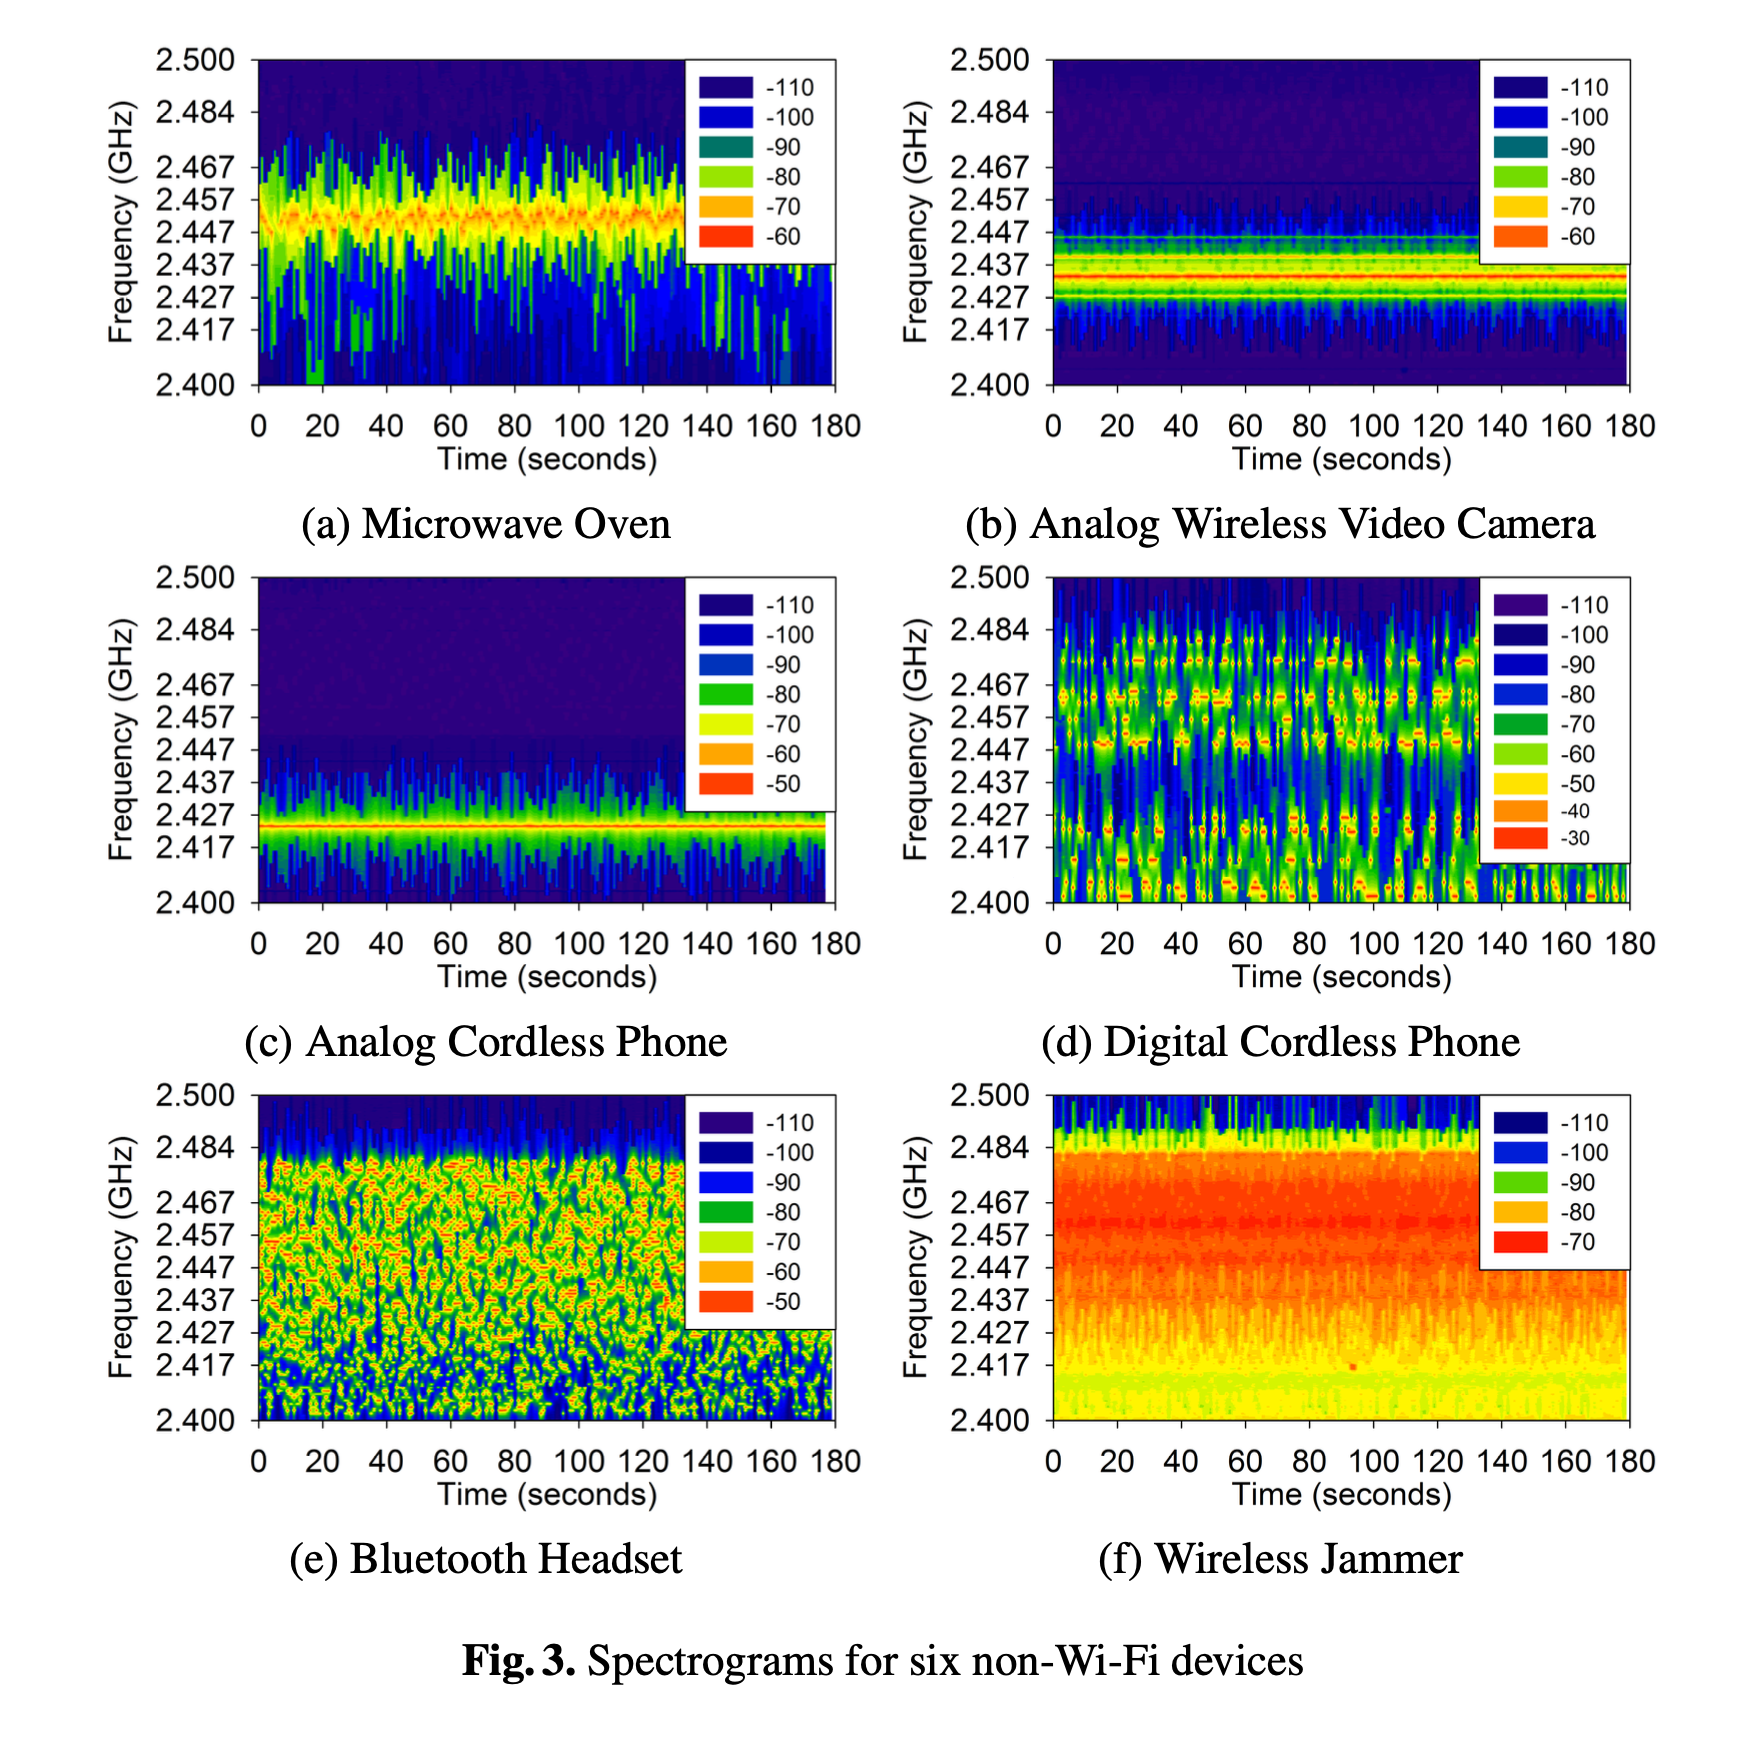
\includegraphics[width=17cm]{res/wifi1.png}
    \caption{实验获得的频谱图}
\end{figure}

图 3 显示了干扰器的频谱图。X 轴代表测量的时间段。Y 轴的刻度线代表偶数 Wi-Fi 信道(即信道 2、4、6、8、10、12 和 14)的中心频率。等值线的颜色代表信号的功率水平,红色表示最强的功率水平,蓝色表示最弱的功率水平。

\subsubsection{功率水平}

干扰源发射的信号强度越高,对Wi-Fi的干扰可能越大。

例如,频谱图中红色代表最强的功率水平,如果红色区域出现在Wi-Fi信道上,说明那个信道受到强烈的干扰。

\subsubsection{频率覆盖}

干扰源影响的频谱范围也代表了干扰源对Wi-Fi的影响。频谱图上的宽带干扰会影响更多的信道,窄带干扰则可能只影响一个或几个信道。

例如,微波炉可能影响多个连续的Wi-Fi信道,而模拟电话可能只影响一个信道。

\subsection{占空比}

\begin{figure}[h]
    \centering
    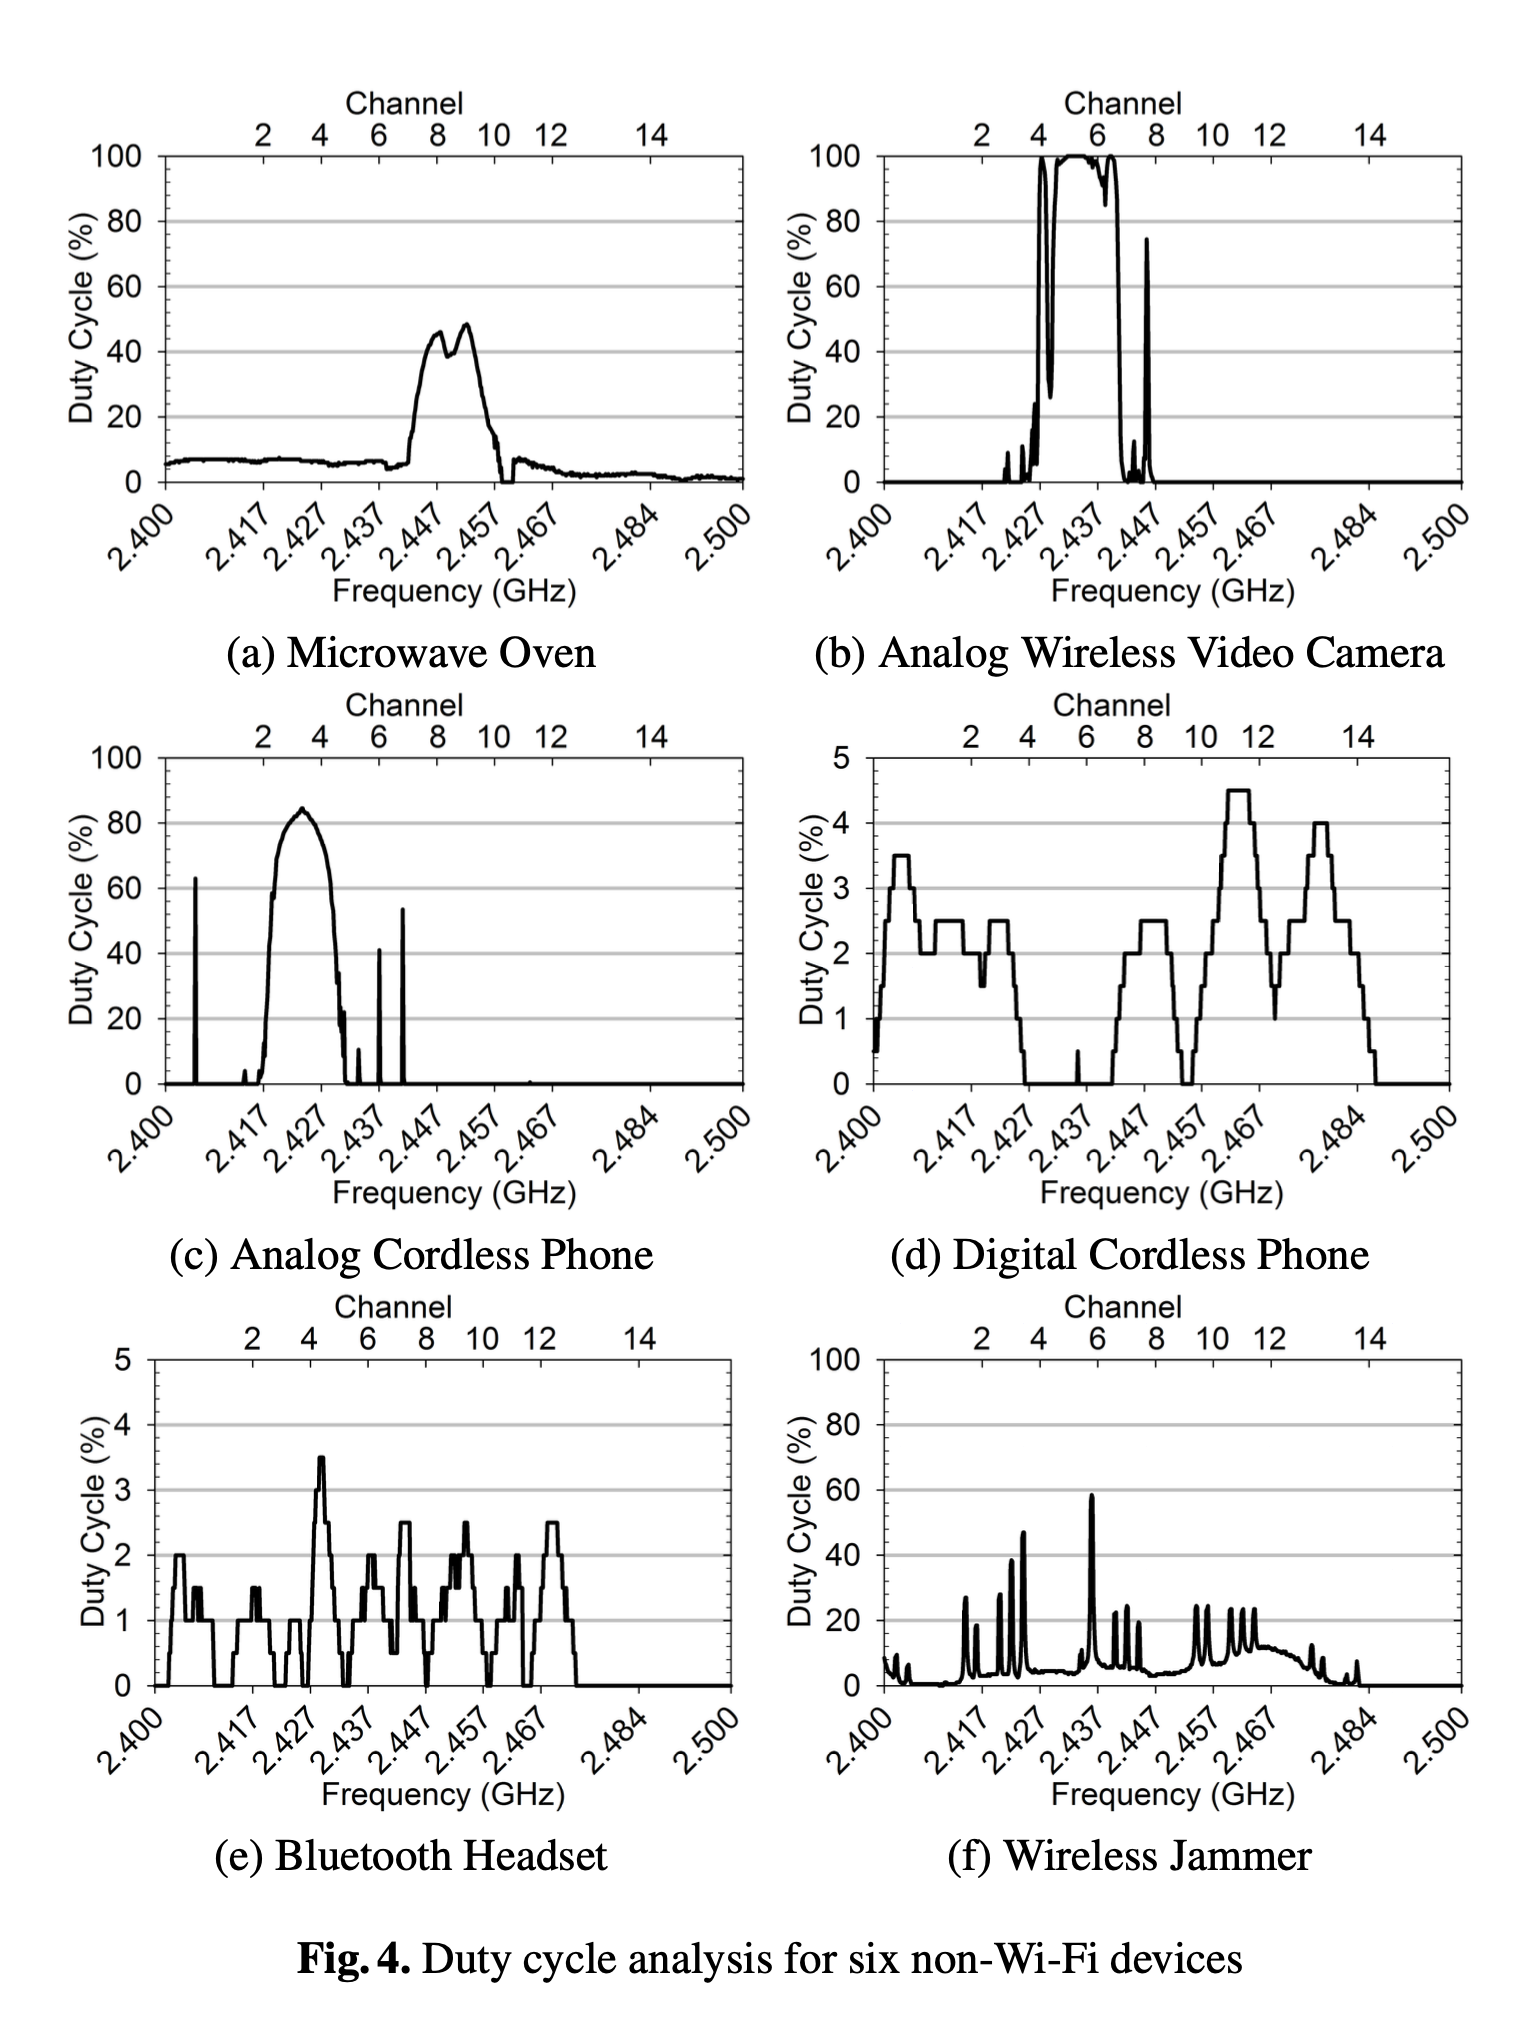
\includegraphics[width=15cm]{res/wifi2.png}
    \caption{实验获得的占空比}
\end{figure}

图 4 显示了干扰器的占空比 FFT 测量结果。X 轴下方的微调标记表示偶数 Wi-Fi 信道的中心频率,而 X 轴上方的微调标记表示与这些中心频率相对应的信道编号。

\subsubsection{高占空比}

高占空比意味着干扰源在大部分时间都在发送信号,这将导致Wi-Fi设备在这些信道上很难进行通信。例如,如果一个设备的占空比接近或等于100\%,则表示它几乎一直在发送信号,会严重影响Wi-Fi设备的使用。

\subsubsection{干扰源的传输特性}

传输特性包括连续传输或跳频(frequency hopping)等技术。连续传输的干扰源可能会持续不断地影响特定信道,而跳频干扰源则可能影响多个信道,但每个信道受影响的时间较短。

\section{基于场景的实验装置分析干扰对数据、视频和语音等各类流量的影响}

在数据实验中,我们使用了吞吐量服务质量(QoS)指标。在视频和语音实验中,我们使用了名为平均意见分数(MOS)的体验质量(QoE)指标。

\begin{figure}[h]
    \centering
    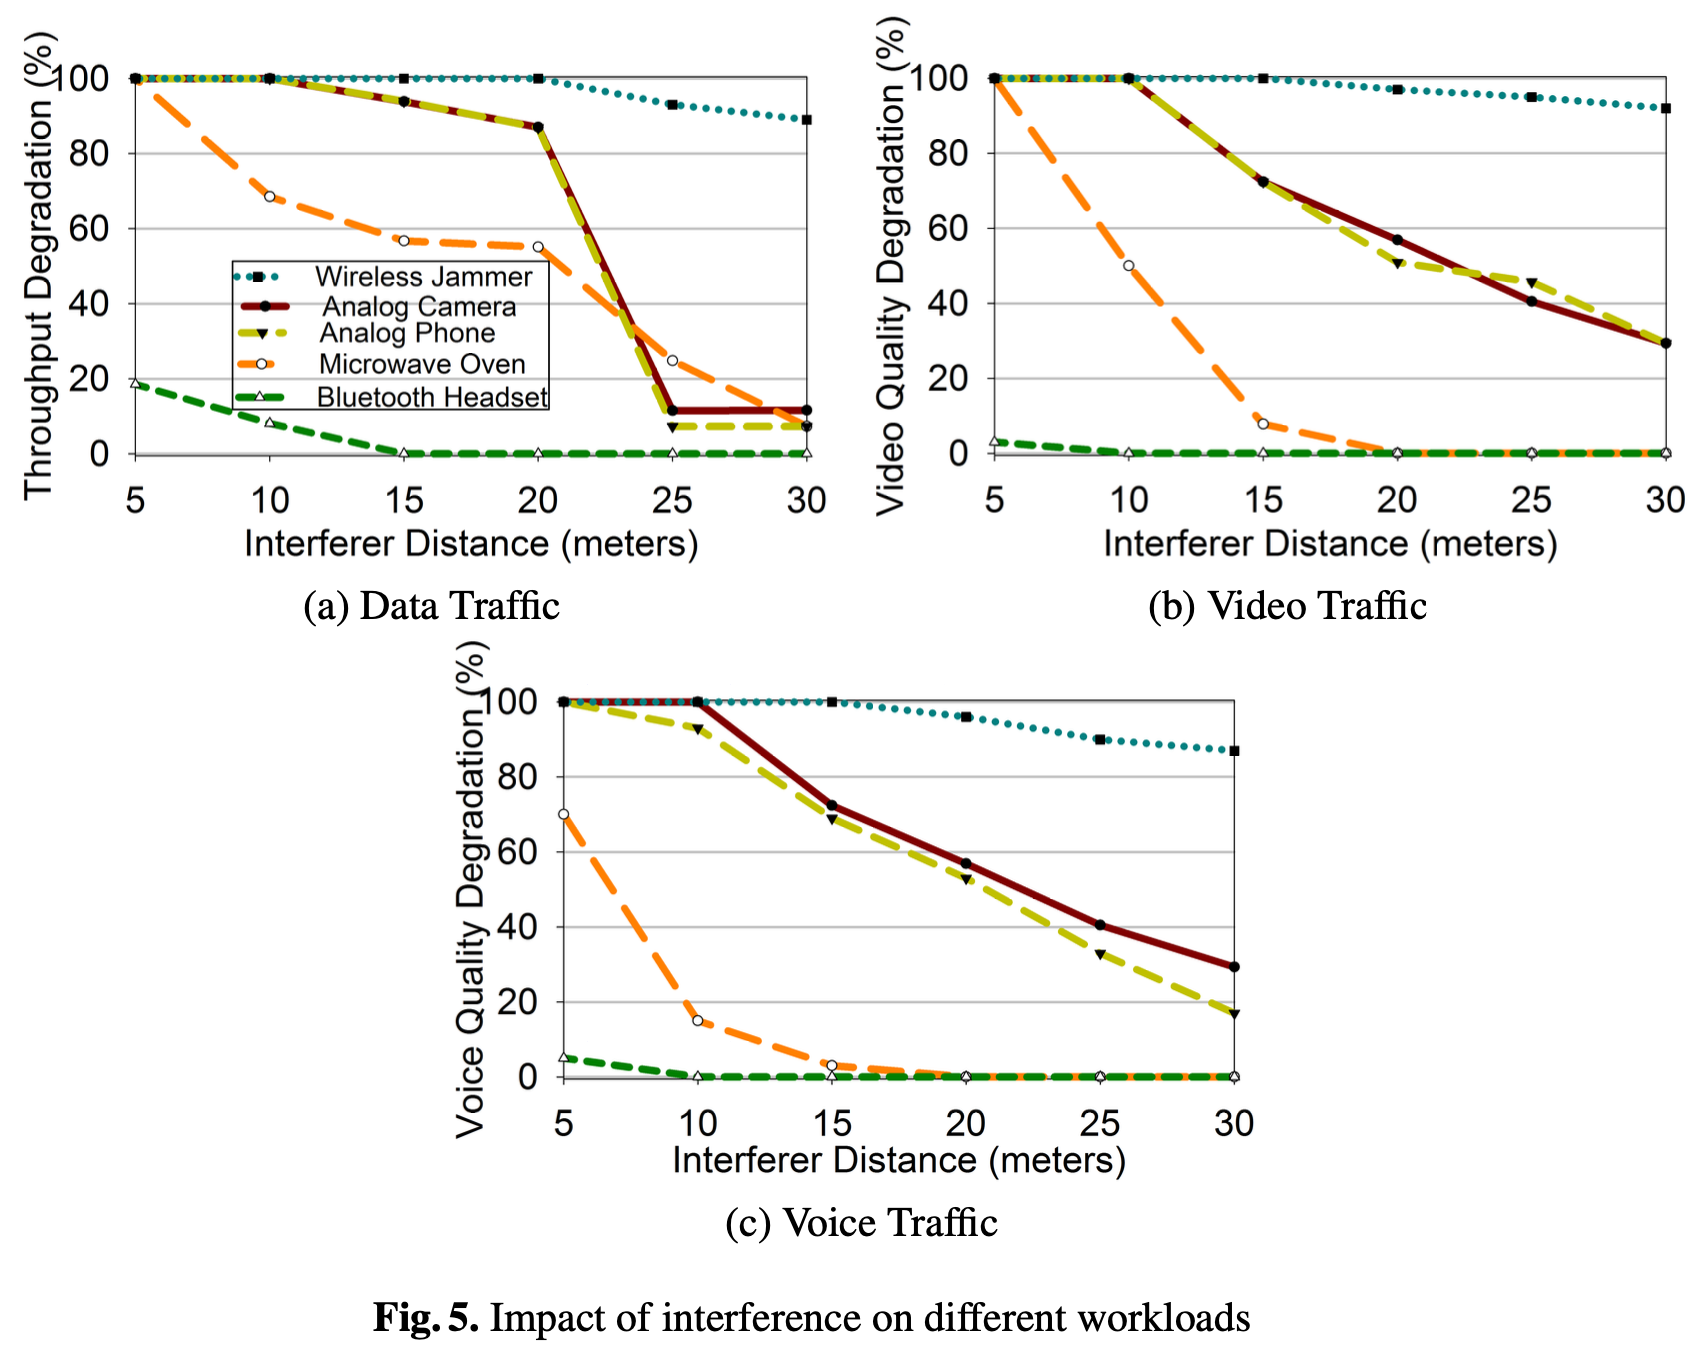
\includegraphics[width=15cm]{res/wifi4.png}
    \caption{实验获得的频谱图}
\end{figure}

不出所料,在使用无线干扰器的实验中,我们始终注意到接近 100\% 的质量下降。这种情况一直持续到 20 米,超过 20 米后,我们观察到其影响略有下降。

\subsection{对数据流量的影响}

使用Iperf工具测量Wi-Fi链路的吞吐量,创建服务器与四个无线客户端笔记本电脑之间的双向TCP流量,持续3分钟。

蓝牙耳机在近距离时减少了20\%的吞吐量。微波炉在近距离时导致吞吐量降至零,即使在25米远的地方也会导致25\%的吞吐量降低。模拟电话和视频摄像头作为连续传输器,在近距离时对吞吐量影响显著,但在超过20米的距离时影响显著减少。

\subsection{对视频流量的影响}

使用伪主观质量评估(PSQA)来计算视频样本的MOS。使用VLC媒体播放器从服务器工作站流式传输3分钟的视频到四个客户端。

蓝牙对视频流量影响最小。微波炉在近距离时严重干扰视频流,远距离时只减少了视频质量的10\%。模拟摄像头和电话对视频流量影响相似,在远距离时视频质量降低了50\%。

\subsection{对语音流量的影响}

记录两人之间3分钟的VoIP对话,将对话双方分成两个音频文件,通过Wi-Fi链路在一对笔记本电脑间进行播放。使用 PSQA 收集语音通信的 MOS 测量值。

语音通信通常使用较小的数据包,对干扰的处理能力最强。

蓝牙在近距离时影响较小,在远距离时几乎没有影响。微波炉在近距离时造成约75\%的退化,但这一数字会随着距离增加而下降。模拟电话和视频摄像头在近距离时影响严重,但随着距离的增加而持续减少,在30米处仍然会造成大约30\%的退化。相比之下,语音流量受干扰的影响较低。

\subsection{一般性结论}

\subsubsection{距离对干扰的影响}

干扰源对Wi-Fi流量的影响通常随着距离的增加而减少。这适用于各种流量类型(数据、视频和语音),其中各类干扰源(蓝牙设备、微波炉、模拟电话和视频摄像头)在远离Wi-Fi网络时对其性能的影响减少。

\subsubsection{干扰源的种类}

不同的干扰源对Wi-Fi流量的影响有显著差异。例如,微波炉在近距离时几乎可以阻断数据流量,而蓝牙耳机对数据流量的影响较小。模拟电话和视频摄像头,作为连续传输器,对流量影响显著,尤其是在近距离。

\subsubsection{不同流量类型对干扰的敏感性}

语音流量因其较小的数据包大小而对干扰的处理能力最好,即便在近距离干扰严重的情况下,其性能下降也不如数据和视频流量。视频流量在某些干扰源下的表现也相对较好,如蓝牙对其影响最小。数据流量在各种干扰下表现最差,特别是在连续传输型干扰源。

\chapter{交通流量}

研究者们使用了在大型大学网络边缘收集的数据包追踪信息来进行分析。他们特别关注了Web和P2P应用在流量级别和主机级别的行为,并试图开发流量级别的分布模型,这些模型可以用于网络仿真和模拟实验,提供对Web和P2P流量相似性和差异性的见解,并洞察当前P2P应用的工作方式。

我们需要了解并计算用于研究互联网流量的主机级和流量级的各种指标。

在跟踪中正确识别 P2P 流量是一个挑战。包括 BitTorrent 和 Gnutella 在内的许多 P2P 应用程序都使用动态端口号。这就需要使用有效载荷签名来识别应用程序。

我们使用开放源代码网络入侵防御系统Bro进行有效负载签名匹配。Bro 内置的有效载荷``签名匹配引擎''用于执行网络流与应用程序类型的映射。我们使用连接建立条件(即 SYN-SYNACK-ACK 数据包传输)或主机间观察到的第一次数据包传输来识别 TCP 流的开始,并在观察到 FIN 或 RST 数据包后识别 TCP 流的结束。默认情况下,如果流量空闲时间超过 900 秒,Bro 就会认为该流量已终止。

\section{流量级别}

为了进行逼真的网络模拟,需要对流量大小、到达间隔时间和持续时间进行建模。

\subsection{流量大小}

流量大小指TCP流量中传输的总字节数。

\subsubsection{Web与P2P}

与 Web 流量相比,P2P 流量的平均流量大小较高,中位流量大小较低。这些观察结果表明,与 Web 相比,P2P 应用程序会产生许多小流量和许多超大流量。P2P 应用贡献了许多小鼠流和大象流,并可能改变了当今 IP 网络中这些流量类型的组合。

小规模流量至少有三个来源:大量信号、传输中止和尝试与无响应的对等方连接。

\subsubsection{Gnutella与比特彗星}

Gnutella 流量比 BitTorrent 流量更大、更分散。这两种应用生成的小流量(例如 5 KB 或更小)所占比例相似。这些较小的流量中有许多是在对等体之间交换控制信息的结果,这是 P2P 协议分布式特性的副产品。

不过,BitTorrent 的大流量占总流量的比例低于 Gnutella。例如,大约 5\% 的 BitTorrent 流量大于 10 KB,而 17\% 的 Gnutella 流量超过了这一大小。Gnutella 似乎比 BitTorrent 产生更多的大流量。BitTorrent 使用文件分割技术将一个对象分割成多个大小相等的块(默认情况下每个块为 256 KB),并使用并行流从相同或不同的对等点下载这些块。相比之下,Gnutella 通常从单个对等点下载整个对象。因此,我们在 BitTorrent 中观察到的大流量比 Gnutella 少。

\subsubsection{老鼠与大象现象}

这两类应用都产生了许多小鼠流量。虽然源自网络应用程序的小鼠流量比源自 P2P 应用程序的小鼠流量少,但网络小鼠流量在网络总字节数中所占的比例相对高于 P2P 小鼠流量在 P2P 总字节数中所占的比例。

两种应用都会产生一小部分大象流量。然而,这些为数不多的 "大象流 "贡献了总字节数的很大一部分。网络运营商可能有兴趣限制这些持续时间较长的 "大象 "流量的带宽,或者有兴趣为这些流量分配较低的优先级。随着 P2P 应用越来越流行,我们可以预见网络将承载越来越多的 "大象 "流。我们的结果还表明,P2P 大象流明显大于网络大象流。

虽然两种 P2P 应用程序的小鼠流比例相似,但 BitTorrent 小鼠流在字节传输中所占的比例远高于 Gnutella 小鼠流;也就是说,Gnutella 小鼠流平均比 BitTorrent 小鼠流小。如前所述,对等点之间的信号传递是 P2P 小鼠流量池的主要成因。我们的数据表明,与 Gnutella 相比,BitTorrent 应用程序的信号活动更频繁,因此小鼠流量相对更大。

尽管 Gnutella 和 BitTorrent 的大象流占字节传输的比例相当,但 Gnutella 的大象流比例远高于 BitTorrent。

一项研究表明,大多数 Gnutella 5 用户分享的主要是音频文件(70\%),而 BitTorrent 用户分享的更多是视频文件(47\%)。平均而言,视频文件要比音频文件大得多。我们认为,超大的 BitTorrent 流量是由于通过单个 TCP 流量传输多个大型视频文件造成的。

\subsubsection{建模}

我们将介绍描述流量大小 (S) 分布的主体和尾部的统计模型。这些模型可用于在网络模拟中生成 TCP 流量的传输大小。图 1 和图 2 描绘了统计模型和经验分布。有界 Weibull 分布和 Pareto 分布的组合很好地模拟了网络流量大小:

\[F_{Web} = 
	\begin{cases} 
       1 - e^{-\left(\frac{S}{2.7}\right)^{0.38}} & : S \leq 30KB \\
       1 - \left(\frac{3}{S}\right)^{1.05} & : 30KB < S \leq 5MB \\
       1 - \left(\frac{200}{S}\right)^{2.35} & : S > 5MB
     \end{cases}
\]

我们发现,Web 流量大小分布的尾部是重尾分布和长尾分布的混合。

同样,我们发现 P2P 流量大小可以很好地用有界 Weibull 和 Pareto 分布来模拟:

\[F_{P2P} = \begin{cases} 
   1 - e^{-\left(\frac{S}{1.36}\right)^{0.81}} & : S \leq 4KB \\
   1 - \left(\frac{0.005}{S}\right)^{0.35} & : 4KB < S \leq 10MB \\
   1 - \left(\frac{400}{S}\right)^{1.42} & : S > 10MB
  \end{cases}\]

根据上述模型,我们可以得出结论:P2P流量大小呈重尾状。

通过结合有界对数正态分布和帕累托分布,Bit Torrent 和 Gnutella 的流量大小都可以很好地建模:

\[F_{BT} = \begin{cases} 
   \Phi \left(\frac{\ln S - 0.03}{0.95}\right) & : S < 2KB \\
   1 - \left(\frac{1.07}{S}\right)^{1.4} & : 2KB \leq S \leq 50KB \\
   1 - \left(\frac{3 \times 10^{-9}}{S}\right)^{0.25} & : 50KB < S \leq 7MB \\
   1 - \left(\frac{0.95}{S}\right)^{0.78} & : S > 7MB
  \end{cases}\]

\[F_{Gnu} = \begin{cases} 
   \Phi \left(\frac{\ln S - 0.44}{0.73}\right) & : S < 3KB \\
   1 - \left(\frac{0.04}{S}\right)^{0.3} & : 3KB \leq S \leq 10MB \\
   1 - \left(\frac{1800}{S}\right)^{1.61} & : S > 10MB
  \end{cases}\]

我们发现,BitTorrent 和 Gnutella 流量大小分布都是重尾分布;但 BitTorrent 流量大小的重尾分布比 Gnutella 流量小。

\subsection{到达间隔时间}

流量到达间隔时间指两个连续流量到达之间的时间间隔。

\subsubsection{Web与P2P}

对数据的分析(见表 5)表明,P2P 流量的到达间隔时间(IAT)比 Web 流量的到达间隔时间(IAT)更长、更分散。Web 流量的到达时间比 P2P 流量的到达时间短得多。例如,约 97\% 的 Web 流量 IAT 小于 0.1 秒,而只有 25\% 的 P2P 流量 IAT 这么短。

了解 Web 流量和 P2P 流量的 IAT 之间差异的另一个方法是研究它们相应的流量到达率。网络流量的到达率较高,约为 80 个流量/秒,而 P2P 流量的到达率仅为 6 个流量/秒。导致 P2P 流量到达率较低和 IAT 值较长的另一个因素是其 TCP 连接的持久性。

关于Web 和 P2P 流量 IAT 的尾部,这两种应用的流量 IAT 在整个尾部显示出类似的衰减。在尾部上端,由于跟踪时间有限,我们观察到急剧衰减。我们发现个别 P2P 应用程序的流量 IAT 也遵循类似的模式

\subsubsection{建模}

略

\subsection{持续时间}

流量持续时间指TCP流量从开始到结束的时间间隔。

Web流通常是短暂的。P2P流则通常是长时间存活的。

\subsubsection{Web与P2P}

存在许多短时流量。大约 30\% 的 P2P 流量持续时间短于 10 秒。这些持续时间较短的传输有些是失败或中止的流量,而其他持续时间较短的流量则是 P2P 应用程序信号行为的副产品。请注意,持续时间短的数据流通常传输少量数据,但反之亦然。有一些持续时间较长的小鼠流;这些流的产生是由于对等方的连接尝试不断失败。我们还观察到,P2P 流量持续时间在 20 到 200 秒之间的占很大比例,约为 40\%。我们发现,一些 P2P 连接受带宽限制,因此持续时间较长。带宽限制反映了对等点之间的可用带宽(例如,不对称互联网接入的对等点上行链路容量有限)以及我们网络上的流量管理(参见第 6 节)。大约 70\% 的网络流持续时间不超过 1 秒。在我们的校园网中,终端用户可以很好地连接互联网,大多数网络服务器的配置也很好。因此,我们预计网络请求的响应时间较短。其余超过 1 秒的网络流通常用于下载大型对象(如从 youtube.com 下载视频流)或使用 HTTP/1.1 持久连接从网页传输多个对象。

我们发现,P2P 流量持续时间长的概率高于 Web。

\subsubsection{Gnutella与比特彗星}

BitTorrent 流量的平均持续时间长于 Gnutella 流量;此外,流量持续时间的取值范围很广。BitTorrent 流量持续时间相对较长的原因在于其协议架构。BitTorrent 采用最稀有的首件选择策略来交换数据。在任何给定时间内,都允许固定数量的并发上传/下载。

BitTorrent 架构允许在对等点之间建立持久连接,并利用其片段选择策略控制下载/上传,从而\textbf{导致连接周期性地处于空闲状态}。此外,从单个 BitTorrent 对等点同时下载会分割上传者用于下载的带宽。相比之下,Gnutella 可使用单一流量下载对象,因此无需共享带宽。Gnutella 对等体偶尔也会共享带宽,例如,当其他对等体请求下载同一对象或同一对等体请求下载不同对象时。

在分布尾部,BitTorrent 流量持续时间比 Gnutella 流量持续时间衰减得更快。我们之前发现,由于 BitTorrent 的文件分割功能,超大流量传输在 BitTorrent 中并不常见。我们还发现,BitTorrent 流量大小与持续时间之间存在正相关关系(相关系数为 0.69),因此观察到 BitTorrent 中超长持续时间流量的比例较低。

其他因素,如文件大小、群组数量和群组中碎片的可用性,也会影响 BitTorrent 流量的持续时间。这些因素导致 BitTorrent 尾部呈长尾状而非重尾状。

\subsubsection{建模}

略。

\section{主机级别}

P2P 流量的主机级特征分析为网络管理员提供了带宽管理和容量规划等任务所需的信息,也为现代 P2P 系统的运行提供了洞察力。本文介绍的结果还可用于开发合成工作负载和设计现实网络模拟。

\subsection{流量并发性}

流量并发性指单台主机同时使用TCP流量传输内容的最大数量。

我们发现,令人吃惊的是,网络中的许多 P2P 主机只维持一个 TCP 连接。网络浏览器通常会启动多个并发连接来并行传输内容。这种并行下载功能增加了基于 HTTP 应用程序的流量并发度。不过,一般的网络客户端通常不会出现高度的流量并发(如超过 30);相反,\textbf{网络代理和内容分发节点才是造成这种高度流量并发的原因。}

大多数 Gnutella 主机每次只连接一台主机。如前所述,Gnutella 应用程序通常使用单个 TCP 流从另一台 Gnutella 主机下载整个对象。我们观察到少数 Gnutella 主机保持着 10 个以上的并发 TCP 连接。这些主机很可能是 Gnutella 对等层中的 "超级对等者"。相比之下,大多数 BitTorrent 主机的流量并发程度较高。大约 24\% 的 BitTorrent 主机使用超过 100 个并发流。这种高度并发是 BitTorrent 的自然现象。BitTorrent 客户端从跟踪器获取对等点列表,然后尝试与这些对等点建立连接。一旦建立连接,BitTorrent 就会使用其最稀有的第一片段选择策略和针锋相对的公平机制来决定如何共享片段。通常情况下,只有少数并发连接会主动传输文件片段。

我们还研究了在一台主机上看到的最大并发流量数与当时连接的不同主机数之间的相关性。并发网络流的数量远远超过了并发连接的网络主机数量。这种行为并不出人意料,因为 BitTorrent 和 eDonkey 等 P2P 协议鼓励与多个主机连接,以促进数据的广泛共享。

\subsection{传输量}

传输量是指在主机活动期间传输到主机和从主机传输的总字节数。上游传输量是指从内部主机传输到外部主机的总字节数。下游传输量是指内部主机从网络外部主机接收的总字节数。

约有一半的 P2P 和网络主机传输少量数据,这些主机的活动时间通常少于 100 秒。这些 P2P 主机反复尝试连接服务对等程序,但都没有成功。连接请求不成功的原因有很多,包括资源不足或所联系的对等端没有有用的内容。与此相反,该区域的网络传输来自网络浏览、定期从网上检索信息的小工具(如天气更新、股票价格)以及下载小文件。

我们发现,大约 35\% 的网络主机和 15\% 的 P2P 主机传输的数据量在 1 到 10 MB 之间,活跃时间大多在 100 到 1000 秒之间。这些 P2P 主机传输数据的原因是共享小物件,而这些网络主机传输数据的原因是长时间浏览网页、下载软件/多媒体文件和基于 HTTP 的流媒体。传输大量数据(如 10 MB 或以上)且活动时间超过 1000 秒的主机比例在 P2P 中明显高于 Web。

\subsubsection{P2P的传输对称性}

传输对称性是 P2P 系统开发者最关心的问题,他们希望鼓励参与的同行之间公平共享。许多内容共享门户网站要求用户保持最低的上游与下游传输量比例,我们称之为最低公平共享比例。

Gnutella 主机的行为似乎以极端的下游和上游传输为主。我们发现,大约 40\% 的 BitTorrent 对等体和 10\% 的 Gnutella 对等体位于公平共享区域。BitTorrent 引入了一种 "针锋相对 "的机制,以鼓励同行之间的公平共享。BitTorrent 系统鼓励每个对等点通过上传获得下载机会。因此,我们在 Gnutella 中看到了更多的 "吃白食者",而在 BitTorrent 中则看到了更好的公平性。


\subsubsection{重量级选手}

我们发现,少数几个主机占据了大部分传输量;我们称这些主机为 "重灾区"。很明显,网络和 P2P 中都有重量级选手。对 P2P 大户的上游与下游传输比率的研究表明,大多数 P2P 大户要么是白吃白喝者,要么是受益者。

排名前 10\% 的网络和 P2P 主机传输的数据总量\textbf{呈幂律分布}($\alpha \approx 0.27$);我们强调,幂律并不适用于排名分布的主体和尾部。

应用之间的唯一区别是总传输量;排名靠前的 P2P 主机传输的数据比排名靠前的 Web 主机多一个数量级。

BitTorrent 重度用户在该应用总字节数中所占的比例远远大于 Gnutella 重度用户在其总字节数中所占的比例。我们还发现,排名靠前的 Gnutella 和 BitTorrent 主机的传输量并不呈幂律分布。

\subsection{地理分布}
地理分布是指单个主机与我们园区之间的最短距离沿地球表面的分布。这种距离测量称为大圆距离(great-circle distance)。

我们使用地理位置数据库计算了单个主机与校园之间的大圆距离。

大部分外部网络主机(约 75\%)位于北美洲;亚洲和欧洲各占外部网络主机的 10\%。这里的结果并不令人吃惊。我们知道,大多数外部网络主机都是网络服务器。我们认为文化上的特殊性也可能会影响结果。我们的大多数校园网用户都讲英语,因此他们更有可能访问以英语为主的国家的网站。

P2P 主机之间的连接似乎并不强烈依赖于主机的位置,而是取决于连接建立阶段的资源可用性。P2P 应用程序的非交互性质使得延迟只是次要问题;首要目标是找到请求的文件。此外,我们的研究结果表明,使用这些系统共享的文件超越了地域界限。

要么 Gnutella 对等者更喜欢连接距离较近的主机,要么 Gnutella 客户端在北美被广泛用于文件共享。我们知道,BitTorrent 主机是从跟踪器提供的对等者列表中连接到对等者的。我们认为,跟踪器提供的列表是根据群组中主机带宽的可用性创建的,因此,我们发现该列表偏向于宽带普及率高的地区。不过,我们确实观察到,尽管 BitTorrent 对等点连接到其他较远的对等点以获取内容,但大多数成功的传输都来自位于同一地理区域的对等点。

\section{一般性结论}

通常情况下,Web 流量的持续时间较短,而 P2P 流量的持续时间较长。网络和 P2P 主机传输都是不对称的;但是,P2P 主机传输主要由上游和下游流量组成,而不是两者都有。网络主机保持高度的流量并发性,而许多 P2P 主机每次只保持一个流量。最后,P2P 流量加剧了互联网流量中的``老鼠和大象''现象。

\part{通信原理}

\chapter{无线通信}

\chapter{蜂窝网络}

\chapter{卫星网络}

\chapter{星链}

\chapter{海底光缆}






\end{document}